\documentclass[11pt]{article}
\usepackage[margin={2cm,2cm}]{geometry}
\usepackage{multicol}
\usepackage{array}
\usepackage{float}
\usepackage{caption}
\usepackage{graphicx}
\usepackage{blindtext}
\newenvironment{Figure}
  {\par\medskip\noindent\minipage{\linewidth}}
  {\endminipage\par\medskip}

\graphicspath{ {/Users/joe/Documents/Masters_Project/NFL-Play-Call-Prediction-with-LSTM-Neural-Networks/paper/figs} }

\setlength{\columnsep}{1cm}

\title{NFL Play Call Prediction Using Sequential Neural Networks}

\author{Joseph W. Director  \\
	University of Colorado Denver \\
    MS Statistics
	\and 
	Joshua French \\
    University of Colorado Denver \\
    Advisor
    \and
    Steffen Borgwardt \\
    University of Colorado Denver \\
    Graduate Committee
    \and
    Florian Pfender \\
    University of Colorado Denver \\
    Graduate Committee
	}

\date{Spring 2022}


\begin{document}

    \pagenumbering{gobble}
    
    \maketitle

    \begin{abstract}
        \centering\begin{minipage}{\dimexpr\paperwidth-12cm}
        The prevelance of data analytics in professional sports has significantly increased over the last 20 years. 
        First popularized in \emph{Moneyball: The Art of Winning an Unfair Game (2003)}, the use of advanced analytics is now mainstream in the four major U.S. sports and abroad. 
        In the National Football League (NFL), millions of dollars are invested into analytics departments and data is being used to drive decision making at every level of an organization's operation. 
        These departments can leverage statistical methods to learn the opposition's tendencies, providing a substantial competitive advantage. 
        In particular, the defensive team can improve its strategy by accurately predicting the offensive team's play call (whether the play is a run or a pass). 
        To this end, many prior works have implemented machine learning algorithms for play call prediction. 
        However, none of the works encountered have treated play-by-play data as sequential. 
        In Football, the offensive team's current play call is dependent upon the sequence of plays called before; therefore, there is a time series component that a modeling strategy must account for. 
        In this work, we explore the ability of sequential deep learning models to predict NFL play calls.
        Namely, we compare the performance of Recurrent Neural Networks (RNNs) and Long Short Term Memory (LSTM) networks to baseline models (Logistic Regression and Gradient Boosted Decision Trees). 
        Using classification accuracy and ROC-AUC as metrics, we found that sequential models out-perform the baseline. 
        \end{minipage}
    \end{abstract}
    
    \pagebreak

    \tableofcontents
    \newpage

    \pagenumbering{arabic}

    \begin{multicols*}{2}
    
    \section{Introduction}

        \subsection{Background}
            
            \paragraph{}
                Gameplay of NFL football is seperated into a sequence of instances called plays. 
                The two teams on either side of the ball are allowed to reposition themselves and prepare in betweeen these instances. 
                Given this nature, there is immense opportunity to strategize when the game is not in play.
                Akin to moving pieces on a chessboard, the coaching staff decides their team's best course of action by anticipating their opponent's moves.  
                For regular plays (i.e. not a kick-off, punt, or field goal attempt), there is a binary option for the type of play the offensive team can do; either a pass or a run.
                A strategic advantage is gained for the defensive team if they can accurately predict this outcome. 
                As a simplistic example, if they predict pass they can put more players in pass coverage, or put more players near the line of scrimmage if they predict run.
            
            \vspace{-10pt}

            \paragraph{}
                There are a number of indicators that can inform play call prediction. 
                Certain personnel packages (groups of players from various positions) and formations of the offensive team are more associated with either passes or runs. 
                Unfortunately, the NFL does not publicly release data containing specific personnel or formations. 
                However, there exists a general binary indicator for the formation; whether the play was from the shotgun (QB lines up a few yards back from the center) or under-center (QB lines up directly behind the center). 
                Beyond this, there is the in-game context of the current play. 
                This includes the down (how many plays can be used to gain the required distance), the distance (the amount of yards needed to gain in order to keep the ball), the score differential, the amount of time remaining, etc. 
                The conditions of these factors all incentivize the offensive team to use either a run or a pass play. 
                For example, if an offensive team is losing by a lot of points with little time remaining in the game, they are more likely to pass because they can gain more yards using less time. 
                Lastly, tendencies of the offensive team can be studied. 
                This is done by accumulating the relative frequency of passes to runs for the offensive team (pass to run ratio) as well as how successful they are at either passing or running (average yards gained per run or pass play).
            
            \vspace{-10pt}
            
            \paragraph{}
                An NFL coach combines experience and intuition to predict the play call. 
                In this work, experience is replaced by labeled data points from the entirety of a single NFL season (2019-2020), and intuition by a supervised machine learning algorithm. 
                A supervised machine learning task involves teaching a computer to learn the underlying patterns relating the response variable to the features. 
                If the model can discern information about the features and response well enough, its predictions should generalize well to unseen instances. 
                A popular domain of machine learning is the field of deep learning. 
                Deep learning uses artificial neural networks (ANNs) that loosely resemble a biological brain. 
                They contain networks of individual neurons or nodes, each with its own activation signal, that is each capable of sending and receiving signals to other nodes (through weights). 
                Types of deep learning algorithms vary in complexity and structure. 
                Here we examine recurrent neural networks (RNNs) and their variant, long short term memory (LSTM) networks. 
                These kinds of networks were originally designed for speech and text recognition because of their ability to learn sequential patterns. 

        \subsection{Problem Statement}
            \paragraph{}
                Prior works have approached play call prediction with machine learning, many implementing complex classification algorithms such as ensemble models and multi-layer perceptrons.
                These methods only provide marginal performance increases from simplistic models such as logistic regression.
                This is because, as is often the case in machine learning tasks, the signal relating the response to the features is only so strong. 
                Therefore, in these cases, the choice of a complex algorithm provides small return as there is little that the added complexity can pick up on.
                Overcoming these performance limits requires rethinking how the data itself is structured.
                In prior approaches, each singular play is treated as a sample point. 
                Treating the data this way means the model isn't aware of any sequential patterns that may exist.
                In the approach proposed by this work, an individual sample point is represented by a play sequence of length $k$. 
        
        \end{multicols*}

        

        
            \begin{table*}[ht]
            \caption{Feature Descriptions} \label{tab:title} 
            \centering
            \begin{tabular}{|| m{4cm} | m{10cm}| m{2cm} ||} 
                \hline
                \textbf{Feature} & \textbf{Description} & \textbf{Type}  \\
                \hline\hline
                Posteam  & Name of team on offense for the current play & Categorical \\
                \hline 
                Defteam & Name of team on defense for the current play & Categorical \\ 
                \hline
                Yardline  & Distance from the goal line (yards) & Numeric \\
                \hline 
                Seconds remaining & Amount of time remaining in current half & Numeric \\
                \hline
                Yards to go & Yards needed to gain for a first down & Numeric \\
                \hline 
                Down & Number of plays to get a first down & Categorical \\
                \hline 
                Shotgun & Whether the offensive team lines up in shotgun formation & Binary \\
                \hline
                No huddle & Whether the offensive team used the huddle before the snap & Binary \\
                \hline 
                Posteam timeouts & Timeouts remaining for offensive team & Numeric \\
                \hline
                Defteam timeouts & Timeouts remaining for defensive team & Numeric \\
                \hline 
                Score differential & Difference in score between offensive and defensive team & Numeric \\
                \hline
                Temperature & On field temperature for the current play & Numeric \\
                \hline 
                Windspeed & On field windspeed for the current play & Numeric \\
                \hline 
                Posteam Home & Whether the offensive team is on its home field & Binary \\
                \hline 
                Half & Whether the play is ran in first or second half & Binary \\
                \hline 
                Dome & Whether the field has a dome or not & Binary \\
                \hline 
                Open & Whether a domed field is open or closed & Binary \\
                \hline 
                Outdoors & Whether the game is played outdoors & Binary \\
                \hline 
                Cumulative run yards & Total yards gained per run play (at current point) & Numeric  \\
                \hline 
                Cumulative pass yards & Total yards gained per pass play (at current point) & Numeric \\
                \hline
                Pass to run ratio & Current proportion of passes ran to total plays & Numeric \\
                \hline
                Pass yards allowed & Total yards allowed per pass play (Defteam) & Numeric \\
                \hline
                Run yards allowed & Total yards allowed per run play (Defteam) & Numeric \\
                \hline
            \end{tabular}
            \end{table*}
        
    \begin{multicols*}{2}
        \subsection{Data}
            \paragraph{}
                Abundant play-by-play data is made easily accessible by the \texttt{nflfastR} package. 
                Data published officially by the NFL is available so no web-scraping is required as a step in preprocessing.
                A singular season (2019) was chosen as the sample because the offensive and defensive teams are used as features; teams are subject to change from year to year. 
                Around 32,000 individual play instances occurred over the course of this season.  
                A list of features chosen for modeling is included in Table 1. 
                Some of these features are given directly by \texttt{nflfastR}, others are acquired through feature engineering.
                The data given is two dimensional $(n,m)$: $n$ samples (individual plays) and $m$ features. 
                These dimensions are fed into baseline models.
                For sequential models, three dimensional data is required $(n,k,m)$: $n$ samples, each sample consisting of $k$ consecutive plays, and $m$ features for each play in the sequence. 
                This requires additional preprocessing.

    \section{Methodology}

        \subsection{Aims}
            \paragraph{}
                Our analysis aims to implement industry standard data science practices for building and testing models.
                This consists of building a scalable data pipeline for preprocessing, hyperparameter tuning, and model selection.
                To this end, cloud computing resources were provisioned from Google Cloud Platform (GCP). 
                This platform allowed for distributed model training on multiple graphics preprocessing units (GPUs); a critical resource given the computational demands of model tuning.  
                The overall workflow for the project is given by Figure 1. 
                Additional steps such as feature engineering and data visualization are included to attain a wholistic view of the data used for modeling.
    
        \end{multicols*}
        \begin{figure}[ht]
            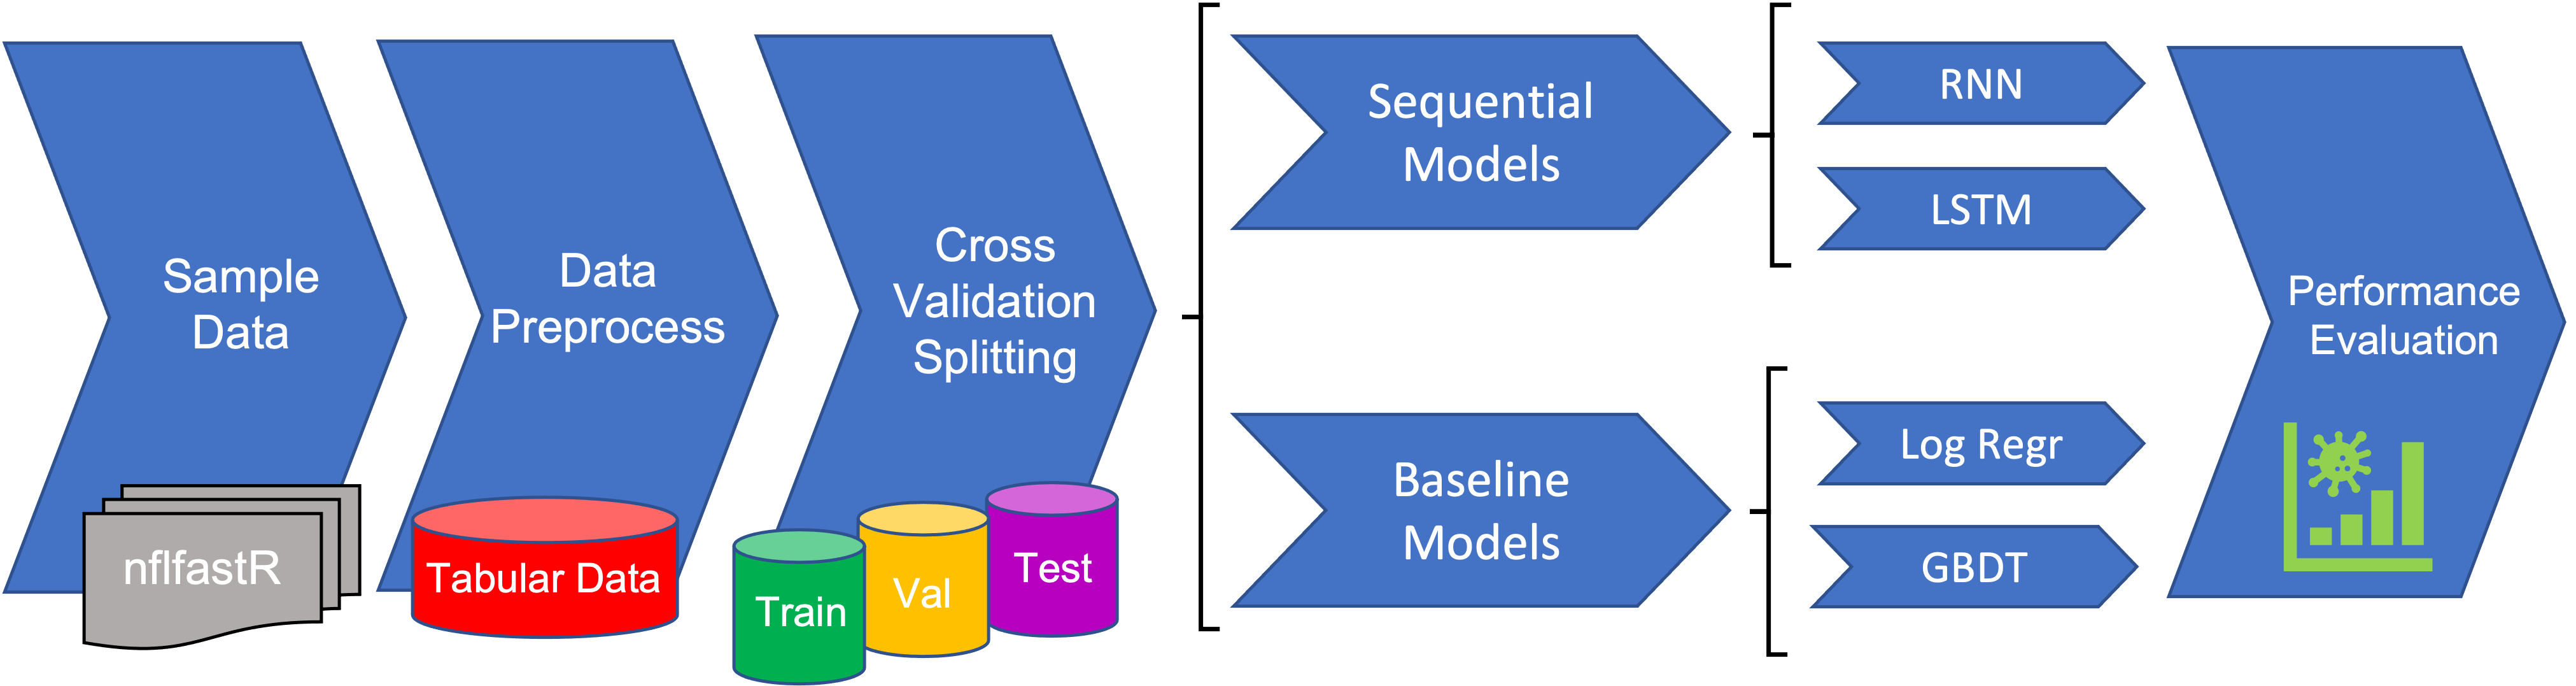
\includegraphics[width = \linewidth]{workflow.png}
            \caption{Overall Methodologic Workflow }
            \label{fig:workflow}
        \end{figure}
        \begin{multicols*}{2}

        \subsection{Preprocessing}
            \paragraph{}
                Data sampled directly from \texttt{nflfastR} contains all play types and outcomes from both the regular and post-season. 
                For the purpose of this analysis, we are only interested in regular season plays that were either passes or runs. 
                This meant removing all instances of special teams plays (kick-offs, punts, field goal attempts) and pre-snap penalties. 
                It is important to note that some plays are intended to be passes but end up being runs (this is called a QB scramble). 
                We consider these to count as passes since this was the intended play call.   
            
        \vspace{-10pt}

            \paragraph{}
                Missing values were only encountered for some of the weather features selected.
                Temperature and wind are NA for games that were played inside of a dome. 
                Inside NFL domes, the temperature is controlled and most often set to 72 degrees fahrenheit.
                Missing values for these features were set to 0 windspeed and 72 degrees fahrenheit for all play instances occurring inside a dome. 
            
        \vspace{-10pt}

            \paragraph{}
                For all methods considered, binary and categorical features need to be one-hot encoded.
                This is because machine learning models aren't able to interperet text strings directly. 
                One-hot encoding entails creating a new column for each level of a categorical variable. 
                The column is a 1 if an instance falls under that category and 0 if not. 
                One-hot endcoding was chosen over integer encoding to avoid creating any ordinal pattern in the categorical features. 
        
        \subsection{Feature Engineering}
            \paragraph{} 
                Feature engineering is a vital aspect of the machine learning process. 
                It is a method by which domain knowledge is leveraged to transform raw data into meaningful features that are capable of distinguishing classes in the response.
                In this case, features are constructed to describe historical tendencies of both the offensive and defensive teams.
                This information is designed to be accurate up until the current play instance. 
            
        \vspace{-10pt} 
            
            \paragraph{}
                Cumulative tendencies are not readily available in data loaded from \texttt{nflfastR}. 
                However, enough information is included in order to build these features. 
                For the cumulative pass to run ratio, we group the data by offensive team and calculate a running total of passes ran divided by total plays. 
                This ensures the feature is current up to a given play; reflecting the information the defensive team would have before the snap. 
                Similarly, we build in features communicating the offensive teams effectiveness at either passing or running.
                The available data includes how many yards were gained for a given play. 
                Again, we group data by offensive team and calculate a runnning total of yards gained (for each type of play) divided by how many plays were ran of that type.  
                 
        \vspace{-10pt}

            \paragraph{}
                In addition to having a sense of the offensive teams tendencies and effectiveness, the defensive team will also be aware of its own weaknesses.
                This aspect is built into the data the same way as offensive tendencies. 
                Instead of grouping by offensive team, we group by defensive team and add a running total of yards allowed per play type.
        
        \subsection{Cross Validation Splitting}
            \paragraph{}
                Cross validation splitting is a method for assessing the performance of a model on unseen data. 
                The original sample of data is partitioned into three non-overlapping subsets called training, validation, and testing.
                Training is used for teaching the model to learn the patterns within the sample. 
                Validation is the first unseen partition and is reserved for evaluating which hyperparameter combinations perform best. 
                Hyperparameters, unlike model parameters, are not learned during the training algorithm and therefore need to be pre-specified by the user.
                Given a number of candidate models performing well on the validation set, a final performance evaluation is done on the testing data. 
                Metrics recorded at this stage are used for final reporting.

            \vspace{10pt}
                
            \begin{Figure}  
                \centering
                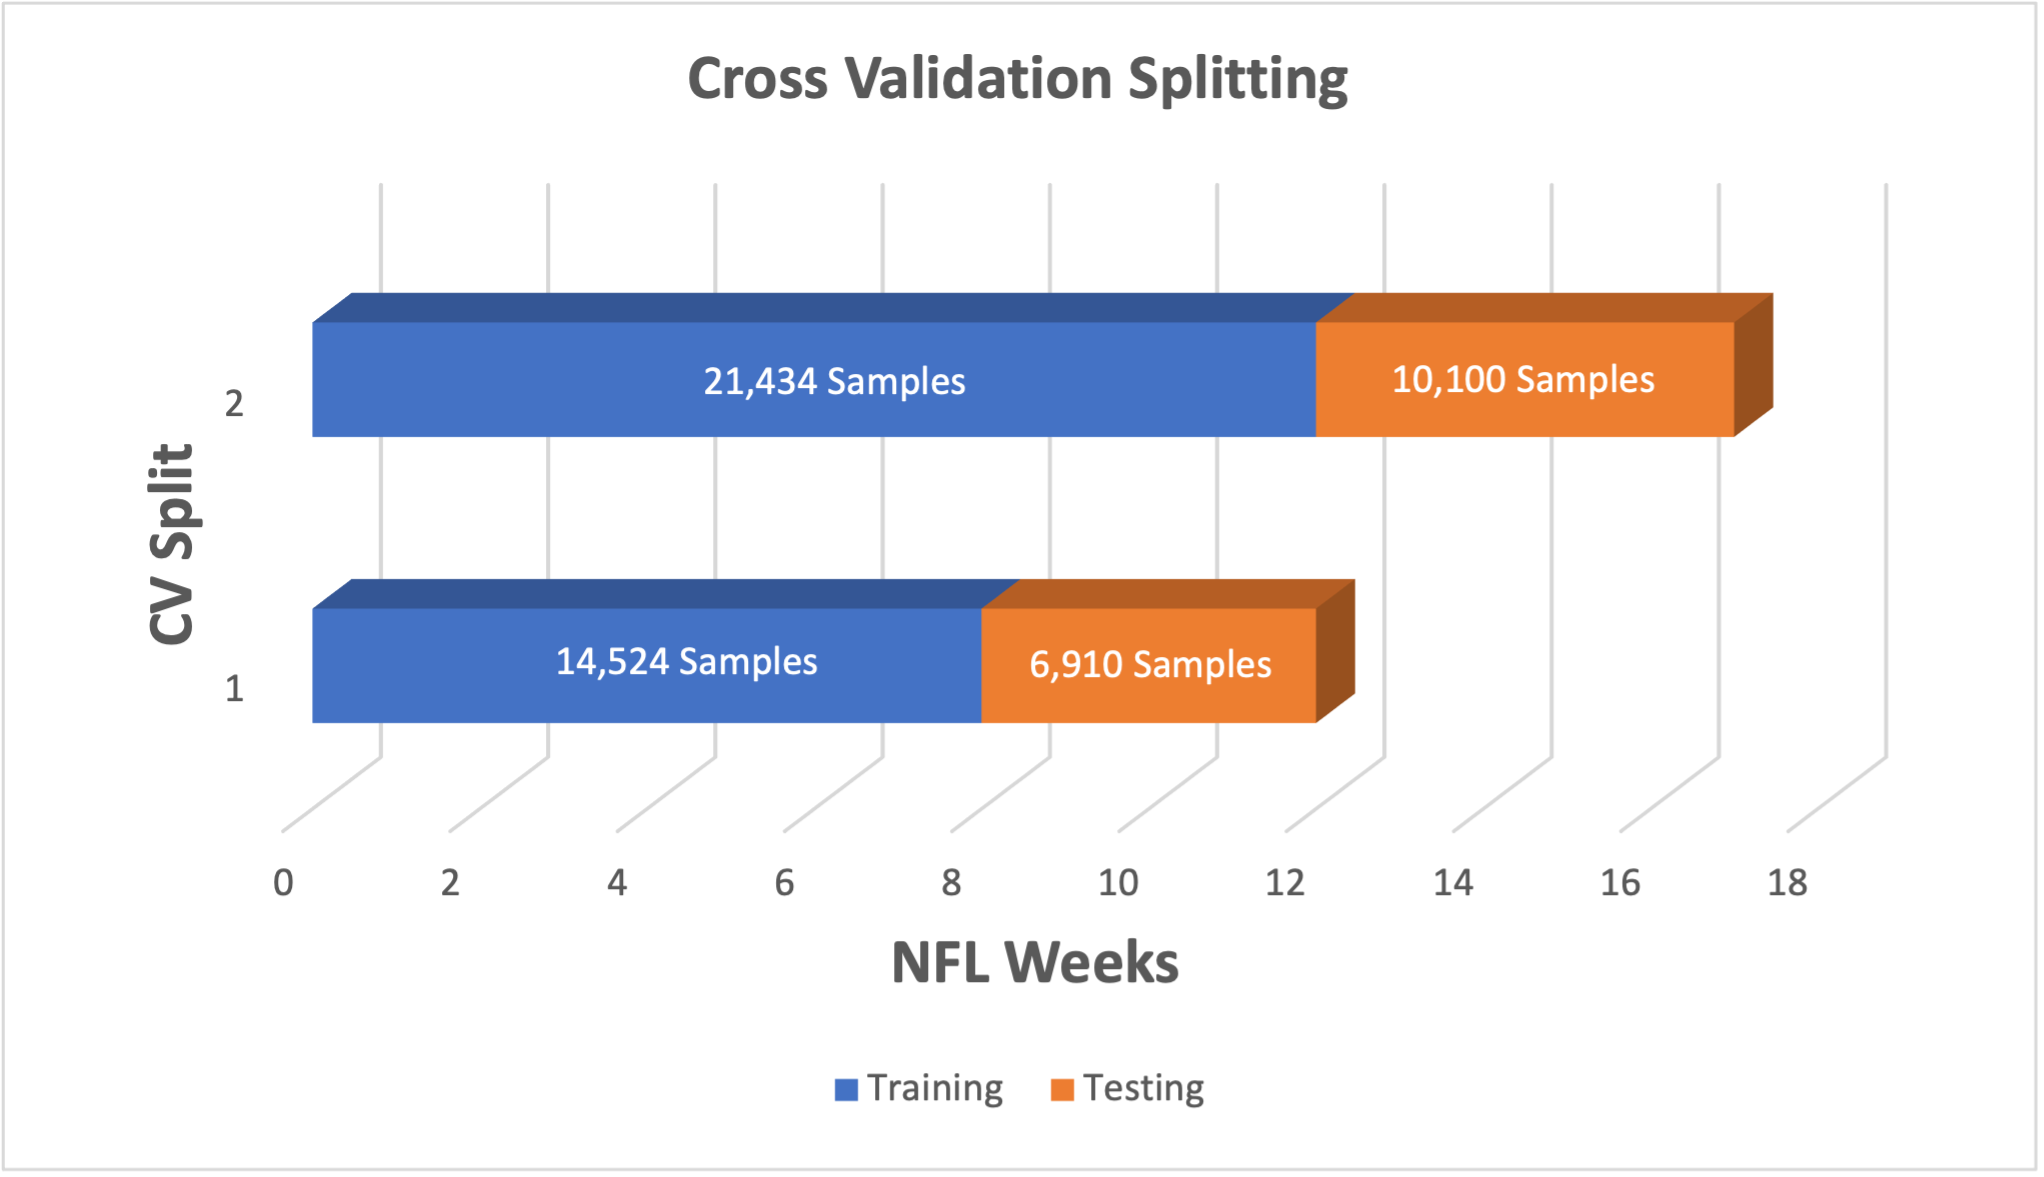
\includegraphics[width = \linewidth]{cv.png}
                \captionof{figure}{Cross Validation Splitting}
                \label{fig:Cross Validation Splitting}
            \end{Figure}

            \vspace{-10pt}

            \paragraph{}
                The cross validation scheme is described in Figure 2.
                The first 8 weeks of the NFL season are used for the training set, with weeks 9-12 as validation for evaluating hyperparameters.
                For each model type, we then select the best 20 hyperparameter combinations for testing. 
                Models with these combinations are retrained using weeks 1-12 and evaluated for final performance using weeks 13-17. 

        \subsection{Exploratory Analysis}
            \paragraph{}
                Exploring the data through table summaries and visualizations is an important step before applying any modeling strategy.
                At this stage, we analyze the distribution of the response variable as well as its relationship to the features.

            \vspace{-5pt}

            \subsubsection*{Response Variable}
                \paragraph{}
                    Understanding the distribution of the binary response variable will inform crucial aspects of applying classification models.
                    Mainly, it gives a sense of the class imbalance. 
                    Class imbalance exists in the data when one of the binary classes occurs much more often than the other. 
                    In cases with heavy imbalance (one class represents 80\% or more the observations), undersampling of the dominant class or oversampling the non-dominant class may need to be applied.
                    Table 2 shows the distribution of the response variable in the different cross validation folds.  
                
                \vspace{15pt}
                
                \begin{tabular}{|| m{2cm} | m{2cm}| m{2cm} ||}
                    \hline
                    \textbf{Fold} & \textbf{\% Pass} & \textbf{\% Run}  \\
                    \hline\hline
                    Train  & 59.50 & 40.5 \\
                    \hline
                    Validation & 60.01 & 39.99 \\
                    \hline
                    Test & 59.01 & 40.99 \\
                    \hline
                \end{tabular}
                \captionof{table}{Play Call Distribution in CV Folds}
                
                \paragraph{}
                    For the three splits, the play call distribution remains at a consistent 60-40 split in favor of passing plays. 
                    This kind of distribution is described as slightly imbalanced data. 
                    No undersampling or oversampling methods are recommended when this is the case. 
                    Note that the overall ratio of passes to runs is the same across the cross validation folds. 
                    The validation data needs to be a representative sample of the training data in order to ensure good results.
            
            \vspace{-5pt}
            \subsubsection*{Features}
                \paragraph{}
                    For brevity, only the most illuminating insights relating play calls to the features are displayed.
                    The first of which is play calls by down and distance, as illustrated in Figure 3. 
                    Notably, it is seen that runs are favored over passes on first downs, second and short, and fourth and short situations.
                    Large disparities between passes and runs exist for third/fourth and 4+ yards as well as second and long scenarios.
                    This matches what is expected as offensive teams are heavily incentivized to throw the ball on later downs and longer distances (need to gain more yards using only one or two plays). 
                    Perhaps the only surprising aspect of the plot is that passes are more common on third and short.
                    A possible explanation is that passes are being ran on third and short when the offensive team already knows it is going to go for it on fourth down (if the third down pass attempt fails). 
                    They are running the riskier option (a pass attempt) knowing they will get another try and then running the safer option (a run attempt) when there is only one attempt available.  

                \end{multicols*}
                \begin{figure}[ht]
                    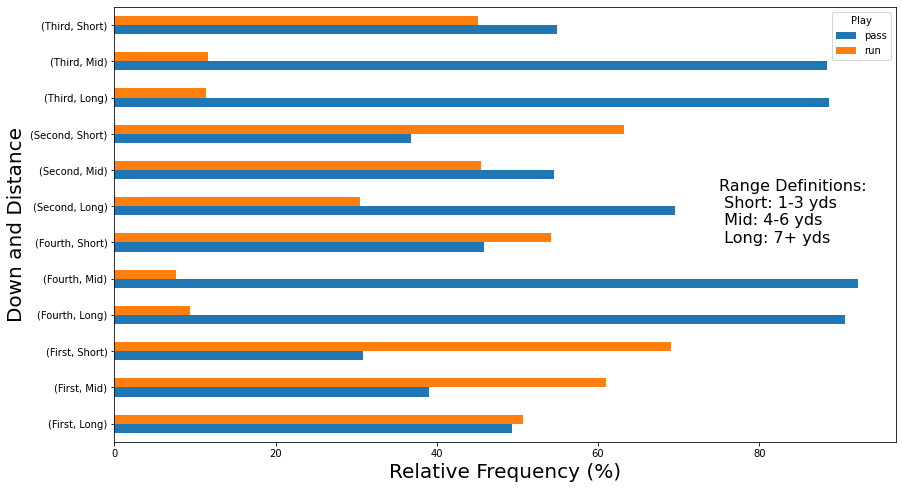
\includegraphics[width = \linewidth]{PlayCallByDownAndDist.png}
                    \caption{Relative Play Call Frequency by Down and Distance}
                    \label{fig:Play Calls}
                \end{figure}
                \begin{multicols*}{2}
                
                \paragraph{}
                    As previously mentioned, there is little information released by the NFL pertaining to what formation the offensive team lines up in.
                    However, they do release whether the play was from the shotgun formation or under center. 
                    In shotgun, the quarterback (QB) lines up farther back from the line of scrimmage. 
                    This is typically to allow more time for the QB to throw the ball before the defensive team can get to him. 
                    The relationship between shotgun formation and play type is displayed by Figure 4. 
                    For more context, the data is grouped by an additional category called huddle.
                    This binary feature tells whether the hurry-up offense is being ran. 
                    In the hurry-up, the offensive team does not meet in a huddle before running the play; this is typically done late in games to avoid losing time in between plays. 
                    The figure confirms what is expected. 
                    Passes are much more common in the shotgun formation and runs are much more common under center. 
                    They remain more common for the hurry-up offense in the shotgun formation but the same result isn't true for under center, huddle plays. 
                    It is suspected more runs are ran in this scenario because these no huddle plays are ran in normal game conditions (i.e. not with little time remaining, down by many points). 

                \begin{Figure}  
                    \centering
                    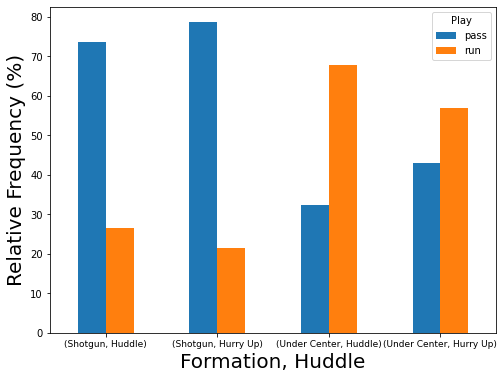
\includegraphics[width = \linewidth]{FormationHuddle.png}
                    \captionof{figure}{Play Frequency by Formation, Huddle}
                    \label{fig:Play Type by Formation and Huddle}
                \end{Figure}

                \vspace{-10pt}
                \paragraph{}
                    There is also some visible tendencies relating score differential and amount of time remaining to optimal play call decisions. 
                    This relationship is explored in Figure 5 where second half plays are examined (so that seconds remaining reflects time left in the game).
                    Passes seem to be called overwhelmingly with less than 500 seconds remaining in the game when a team is down by 0-20 points. 
                    During this same time window, runs seem to be called more when a team is leading by 0-20 points.
                    
                    \end{multicols*}
                    \begin{figure}[ht]
                        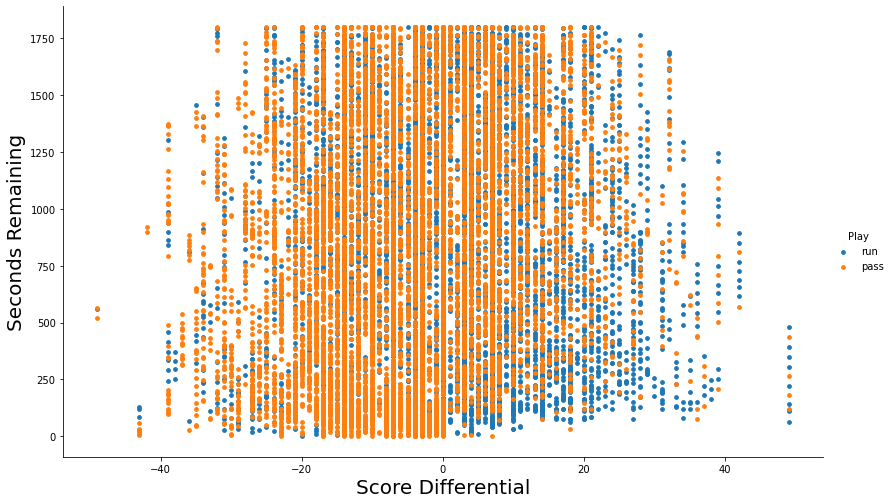
\includegraphics[width = \linewidth]{ScoreDiffSecRem.png}
                        \caption{Play Call by Score Differential and Seconds Remaining}
                        \label{fig:Play Call by Score Differential and Seconds Remaining}
                    \end{figure}
                    \begin{multicols*}{2}

                \paragraph{}
                    Finally, the evolution of play call tendencies as the season progresses are visualized in Figure 6. 
                    Teams are plotted by division (across conferences) for added visual clarity.
                    The behavior for each team is generally sporaditic for the first 1000-2000 play calls. 
                    Beyond this threshold, a given team's overall tendencies begin to steady out. 
                    In the long run it is seen that all teams operate by using around 40-80\% passing plays with most teams using about 60\%. 
                    This matches the play call distributions seen in Table 2.
                    
        
        \subsection{Sequential Models}
            \paragraph{}
                Mathematical details for the sequential neural networks used in this analysis are given. 

            \vspace{-5pt}

            \subsubsection*{Recurrent Neural Networks}
                \paragraph{}
                    Recurrent neural networks are a special class of artificial neural networks where connections between nodes flow in a consecutive sequence. 
                    This allows them to exhibit memory-like behavior and learn to understand temporal patterns. 
                    While originally intended for speech and text recognition, they have been applied to a multitude of tasks where data represents a time series.
                
                \vspace{-10pt}

                \paragraph{}
                    For the models used in this work, let the pair $(X_i, y_i)$ for $i = 1,2,...N$ represent a training observation where:
                    
                    \begin{itemize}
                        \item $X_i := X_{t-k}^l, X_{t-k+1}^l, ... , X_{t}^l$ i.e. a sequence (size $k$) of design vectors (dimension $l$, the number of features)  
                        \item $y_i := y_{t}$ i.e. the binary response at time $t$ 
                    \end{itemize}

                    Importantly, each input represents a sequence of feature vectors of length $k$ while the target is the binary label at the end of each sequence. 
                    Hence, in the context of this analysis, the previous $k$ play calls and current conditions are used to predict the play at timestep $t$. 
                    Now define a simple recurrent network connecting the sequence of inputs to the outputs:

                    \begin{itemize}
                        \item $h_i = \sigma_{h}(W_{h}X_{i} + U_{h}h_{i-1} + b_{h})$ 
                        \item $\hat{y_i} = \sigma_{y}(W_{y}h_{i} + b_{y})$ 
                    \end{itemize}

                    Where $X_i$ is defined as above and the rest are given by:



            \end{multicols*}
            \begin{figure}[ht]
                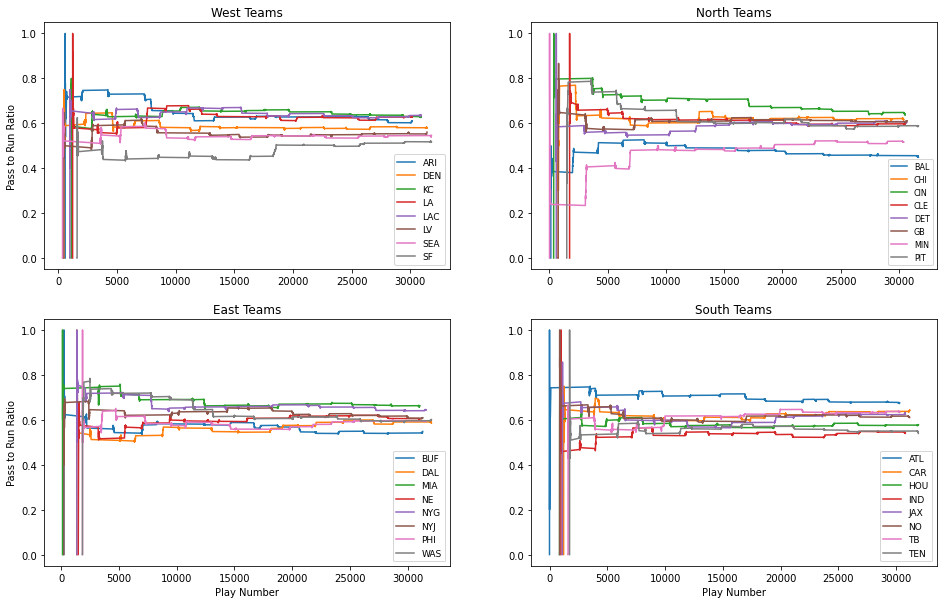
\includegraphics[width = \linewidth]{ptr.png}
                \caption{Pass to Run Ratio by Team}
                \label{fig:Pass to Run Ratio by Team}
            \end{figure}
            \begin{multicols*}{2}

                    \begin{itemize}
                        \item $h_i := $ Vector of hidden states
                        \item $W_h := $ Weights connecting input to hidden state
                        \item $U_h := $ Weights connecting hidden state to previous hidden state 
                        \item $b_h := $ Hidden state biases
                        \item $W_y := $ Weights connecting hidden state to output
                        \item $b_y := $ Output biases
                        \item $\sigma_h := $ Hidden state activation function
                        \item $\sigma_y := $ Output activation function
                        \item $\hat{y_i} := $ Predicted target variable
                    \end{itemize}

                \paragraph{}
                    A visual representation of the network is given in Figure 7.
                    
                      

                     

      


                    



\end{multicols*}
\end{document}